\section{Wie die Welt in den Computer kam – Narrative der Technikgeschichte}

\subsection{Einführung: Computergeschichte als Erzählung}

Die Sitzung beginnt mit einer populären Computergeschichte (Film). 
Bereits hier wird deutlich: Computergeschichte ist nie nur eine Abfolge technischer Innovationen, 
sondern immer auch eine \textit{Erzählung}.

Zentrale Leitfragen:

\begin{itemize}
    \item Was wird erzählt – und was wird nicht erzählt?
    \item Wer erscheint als Erfinderfigur?
    \item Welches Problem soll der Computer lösen?
    \item Was ist überhaupt ein Computer?
\end{itemize}

Computergeschichte ist somit nicht neutral, sondern konstruiert Bedeutungen, 
setzt Schwerpunkte und lässt andere Aspekte verschwinden.

\subsection{Etappen der Computergeschichte}

Die Vorlesung strukturiert die Geschichte des Computers in fünf Phasen:

\begin{enumerate}
    \item Vorläufer bis 1900
    \item 1930er/1940er: Militär und Wissenschaft
    \item 1950er/1960er: Kommerzielle Verwaltungsmaschinen
    \item 1970er/1980er: Computer für alle
    \item Ab 1990: Computer als Infrastruktur und Umwelt
\end{enumerate}

Diese Periodisierung zeigt, dass sich nicht nur die Technik, sondern auch 
die gesellschaftliche Funktion des Computers verändert.

\subsection{1. Vorläufer bis 1900}

\begin{center}
    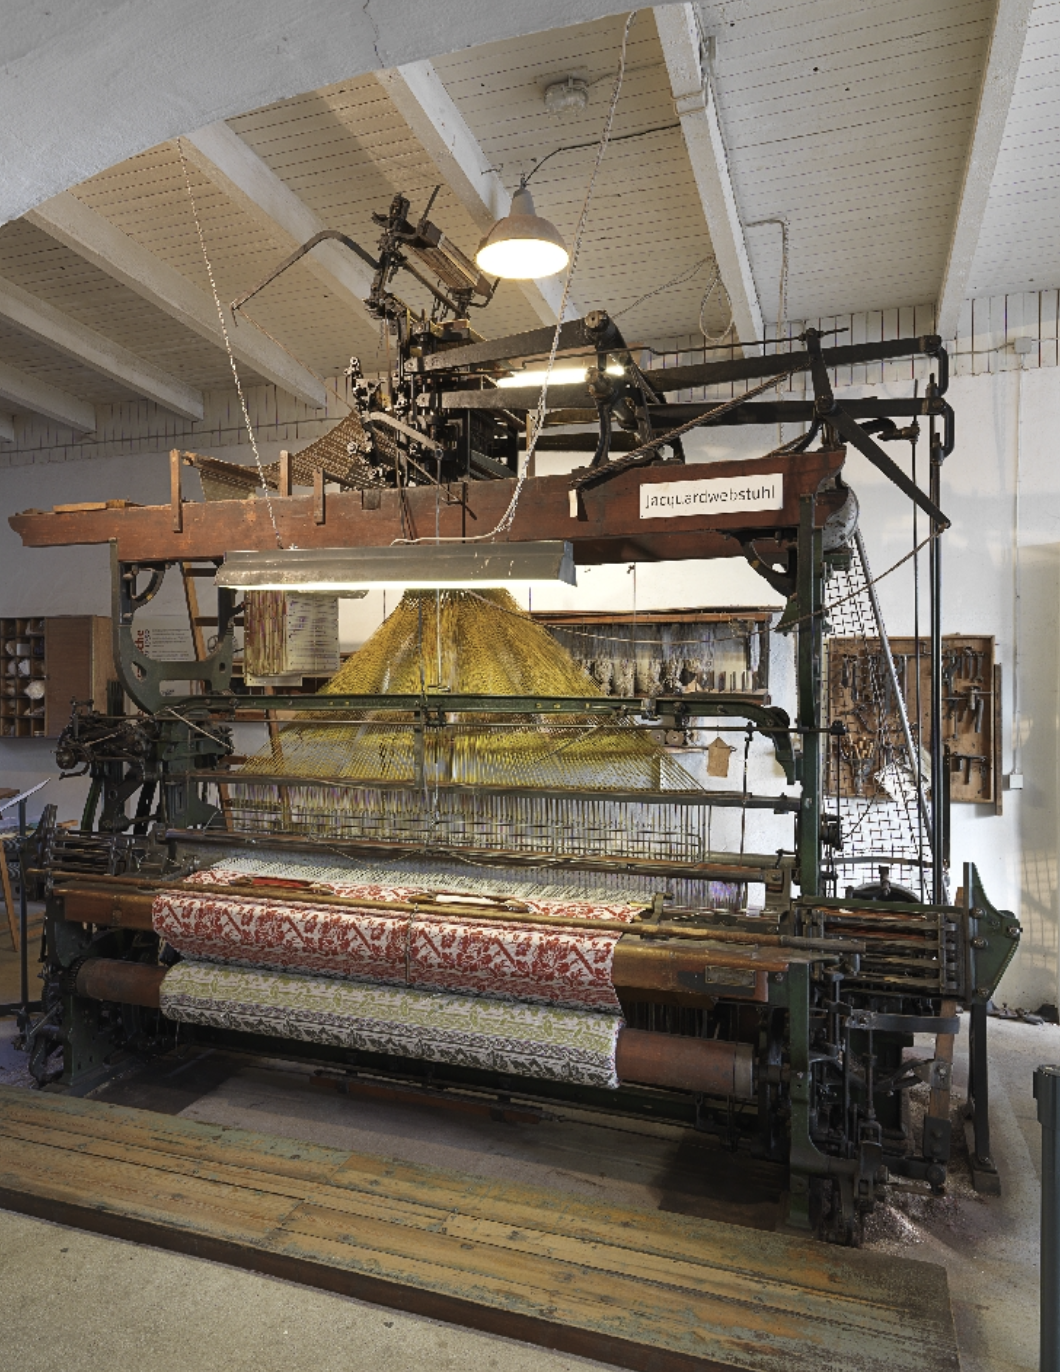
\includegraphics[width=0.8\linewidth]{images/jacquardwebstuhl.png}
\end{center}

\begin{center}
    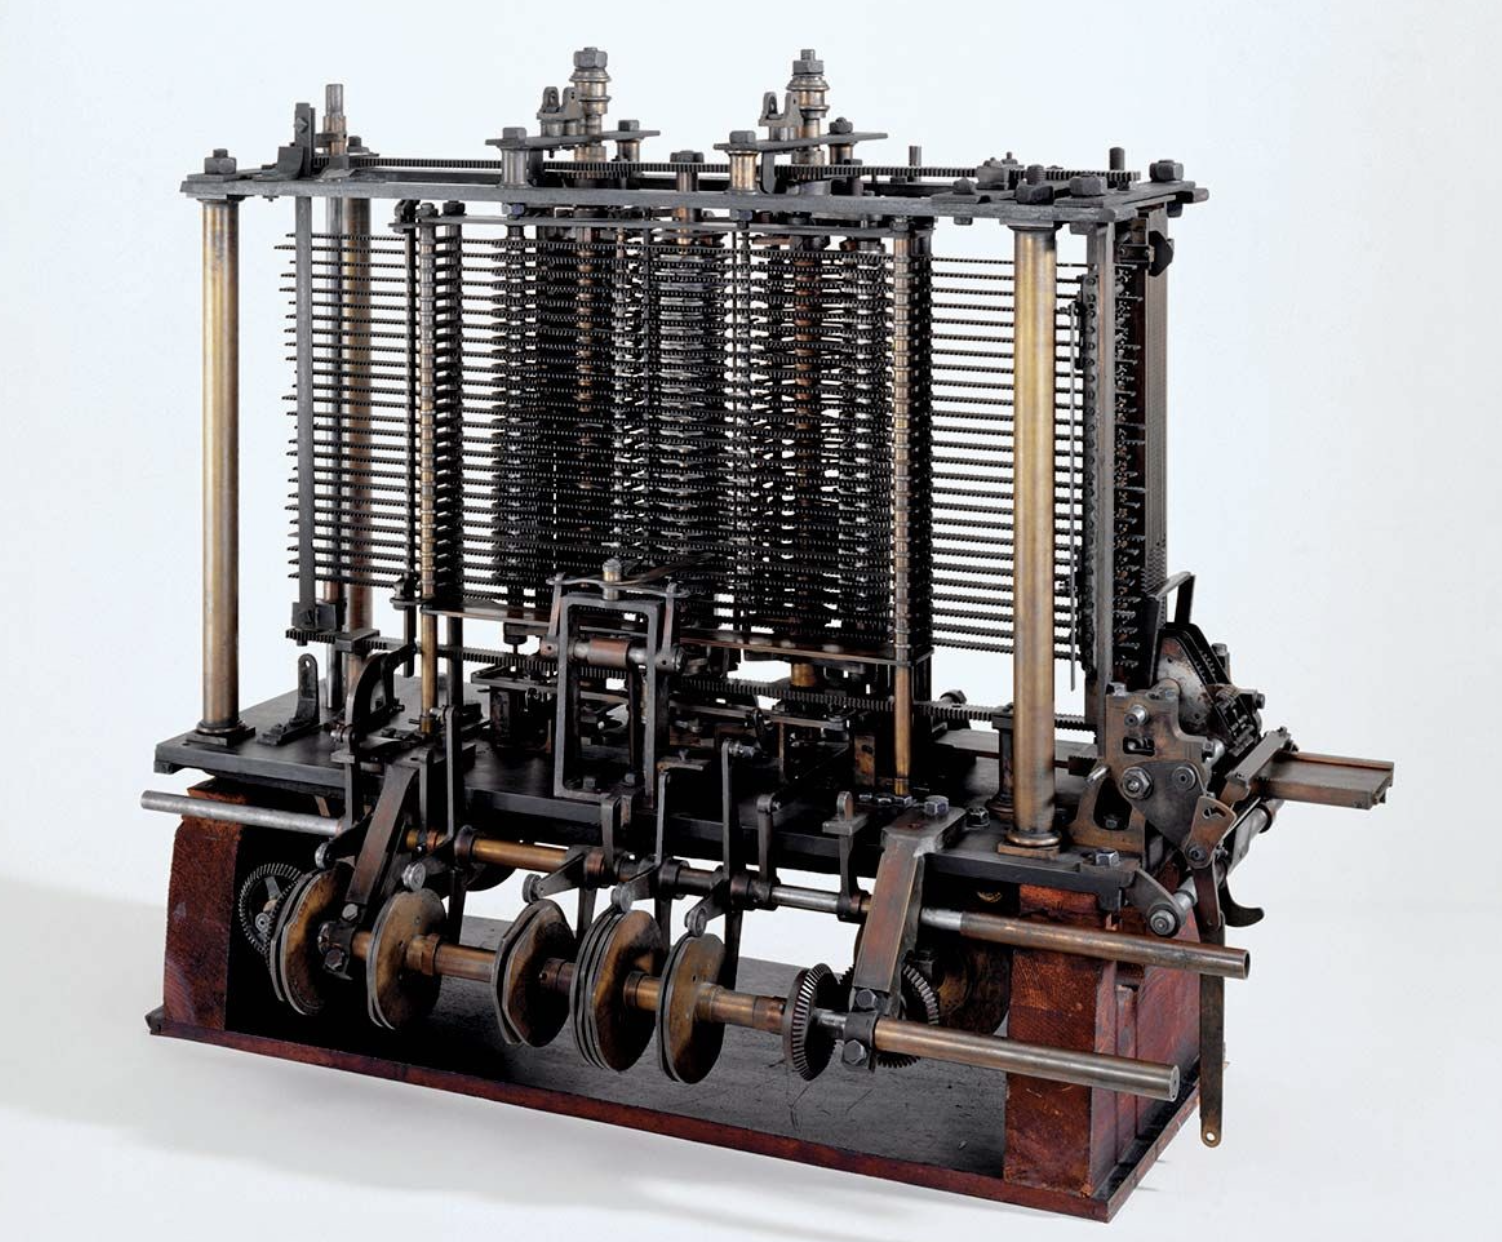
\includegraphics[width=0.8\linewidth]{images/analyticalmachine.png}
\end{center}

Die frühen Vorläufer waren keine „Computer“ im heutigen Sinn, 
sondern Maschinen zur Automatisierung bestimmter Prozesse.

\paragraph{Jacquardwebstuhl (um 1800)}

\begin{itemize}
    \item Automatisierung komplexer Webmuster
    \item Steuerung über Lochkarten
    \item Industrielle Anwendung
\end{itemize}

Hier wird erstmals das Prinzip sichtbar, dass ein Programm 
von der Maschine getrennt existieren kann.

\paragraph{Analytical Machine (Babbage/Lovelace, 1840er)}

\begin{itemize}
    \item Dampfbetrieben
    \item Lochkarten
    \item Allgemeine Programmierbarkeit
    \item Theoretisches Konzept, nicht realisiert
\end{itemize}

Die Analytical Machine formulierte bereits das Prinzip eines 
universellen Rechners.

\paragraph{Hollerith-Maschinen (um 1900)}

\begin{itemize}
    \item Lochkartenbasiert
    \item Verarbeitung grosser Datenmengen
    \item Einsatz bei Volkszählungen
    \item Verwaltungsmaschine
\end{itemize}

Hier verschiebt sich der Zweck: weg von mathematischen Problemen, 
hin zur Datenverarbeitung im administrativen Kontext.

Gemeinsames Prinzip dieser Vorläufer:
Die Trennung von Maschine und Programm ermöglicht 
eine Zweckungebundenheit des Rechners.

\subsection{2. 1930er und 1940er: Militär und Wissenschaft}

Mit der Elektrifizierung entstehen elektronische und elektromechanische Rechner.

Beispiele:

\begin{itemize}
    \item Konrad Zuse (Z4)
    \item Colossus (Grossbritannien)
    \item ENIAC (USA)
\end{itemize}

Der Computer wird zur Kriegstechnologie.

Zwecke:

\begin{itemize}
    \item Ballistische Berechnungen
    \item Kryptographie
    \item Entwicklung der Atombombe
\end{itemize}

Charakteristisch:

\begin{itemize}
    \item Massive staatliche Investitionen
    \item Geheimhaltung
    \item Nationale Sicherheit als Legitimation
\end{itemize}

Der Computer ist nun strategisches Instrument.

\subsection{3. 1950er/1960er: Kommerzielle Verwaltungsmaschinen}

\begin{center}
    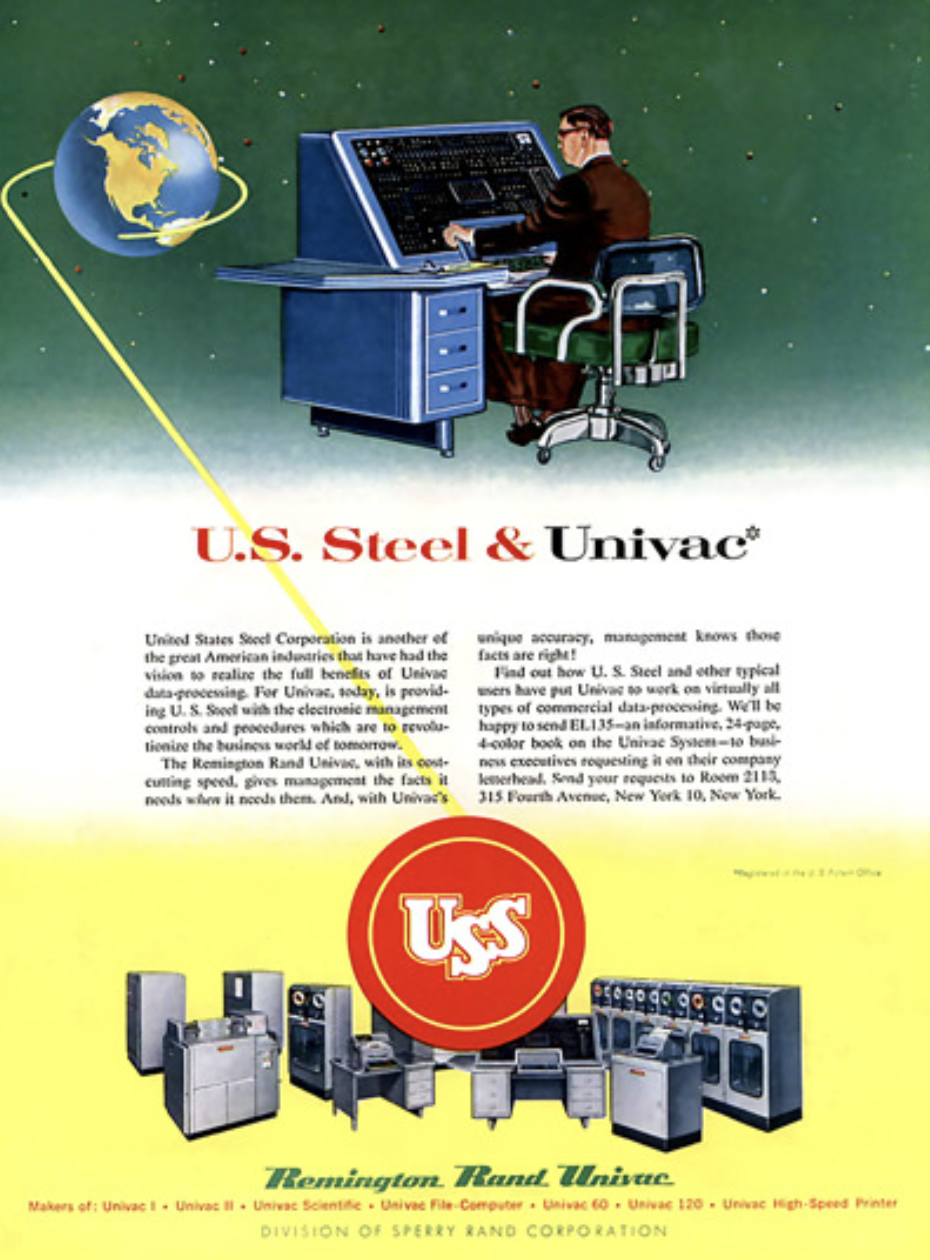
\includegraphics[width=0.8\linewidth]{images/univacwerbung.png}
\end{center}

Mit UNIVAC (1951) beginnt die kommerzielle Phase.

\paragraph{Mainframes}

\begin{itemize}
    \item Raumfüllende Grossrechner
    \item Installation in Rechenzentren
    \item Nutzung durch Banken, Versicherungen, Verwaltungen
\end{itemize}

Zweck:
Effizienzsteigerung bürokratischer Prozesse.

\paragraph{Datenverarbeitung}

Der Prozess war komplex:

\begin{enumerate}
    \item Daten erfassen (Digitalisierung)
    \item Programm schreiben
    \item Lochkarten stanzen
    \item Im Rechenzentrum einreichen
    \item Warten (Stapelverarbeitung)
    \item Resultate abholen
\end{enumerate}

Probleme:

\begin{itemize}
    \item Hohe Kosten
    \item Vermeidung von „idle time“
    \item Unflexible Stapelverarbeitung
\end{itemize}

\paragraph{Technische Lösungen}

\begin{itemize}
    \item Random Access (Magnetplatten statt Magnetband)
    \item Time-Sharing (Mehrere Terminals, quasi Echtzeit)
\end{itemize}

Folgen:

\begin{itemize}
    \item Flexibilisierung des Datenzugriffs
    \item Grundlage für Datenbanksysteme
    \item Beginn der Vernetzung
\end{itemize}

\subsection{4. 1970er/1980er: Computer für alle}

Mit dem Mikroprozessor werden Computer kleiner, billiger und leistungsfähiger.

Es entstehen:

\begin{itemize}
    \item Personal Computer
    \item Vernetzungstechnologien
    \item Neue Firmen im Silicon Valley
\end{itemize}

Die Erzählung ändert sich:
Computer werden als Mittel zur Demokratisierung inszeniert.

Gleichzeitig:

\begin{itemize}
    \item Standardsoftware reguliert Nutzungsmöglichkeiten
    \item Benutzeroberflächen verdecken technische Komplexität
\end{itemize}

Hackerkulturen (z.B. Chaos Computer Club) reagieren kritisch und fordern 
Datenschutz und Transparenz.

Technik tritt zunehmend in den Hintergrund.

\subsection{5. Ab 1990: Computer als Infrastruktur und Umwelt}

Mit dem Internet verschwindet der Computer als einzelnes Gerät 
und wird Teil einer globalen Infrastruktur.

\begin{itemize}
    \item Tim Berners-Lee entwickelt das World Wide Web
    \item Browser (Mosaic, Netscape) machen es zugänglich
    \item Suchmaschinen strukturieren Daten
\end{itemize}

Neu ist:

\begin{itemize}
    \item Verkauf digitaler Dienstleistungen
    \item Plattformökonomie (Amazon, Google, Facebook)
    \item Daten als Zahlungsmittel
\end{itemize}

Der Computer wird unsichtbar – er wird zur Umwelt.

Zentrale Frage:
Was ist ein Computer noch, wenn er überall ist?

\subsection{Zentrale Erkenntnisse}

Die Geschichte des Computers ist keine lineare Erfolgsgeschichte.

Sie zeigt:

\begin{itemize}
    \item Verschiebung der Zwecke (Rechnen → Verwaltung → Kommunikation → Infrastruktur)
    \item Veränderung der Akteurskonstellationen (Privatpersonen → Militär → Konzerne → Plattformen)
    \item Wandel der Wahrnehmung (sichtbare Maschine → unsichtbare Infrastruktur)
\end{itemize}

Computergeschichte ist daher immer auch:

\begin{itemize}
    \item Militärgeschichte
    \item Verwaltungsgeschichte
    \item Wirtschaftsgeschichte
    \item Kulturgeschichte
    \item Infrastrukturgeschichte
\end{itemize}

Die zentrale These lautet:

Nicht nur der Computer hat sich verändert – 
auch das, was als „Computer“ gilt, hat sich historisch gewandelt.
